\chapter{MAD-GAN Results}\label{apdx:madgan_res}
Results of the MAD-GAN approach for anomaly detection in solar wind profiles. Two models were created, one for detecting input variables and the other for the outputs. Each model produces an anomaly score for every file in the dataset and a defined percentage is considered anomalous. In these experiments the threshold is set at 3\%.

\section{Input Model}

\begin{figure}[h]
    \centering
    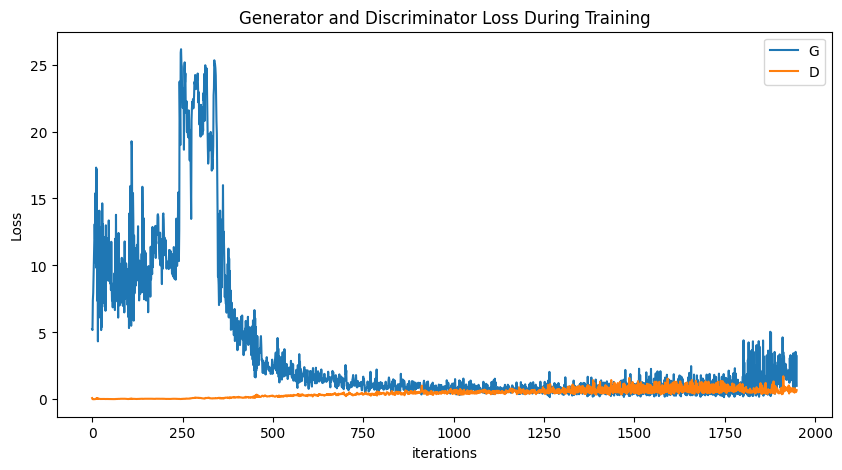
\includegraphics[width=0.8\textwidth]{figures/madga_train_hist_in.png}
    \caption{MAD-GAN input model training history.}
    \label{fig_a:madgan_in_hist}
\end{figure}

\begin{figure}
    \centering
    \rotatebox[origin=c]{-90}{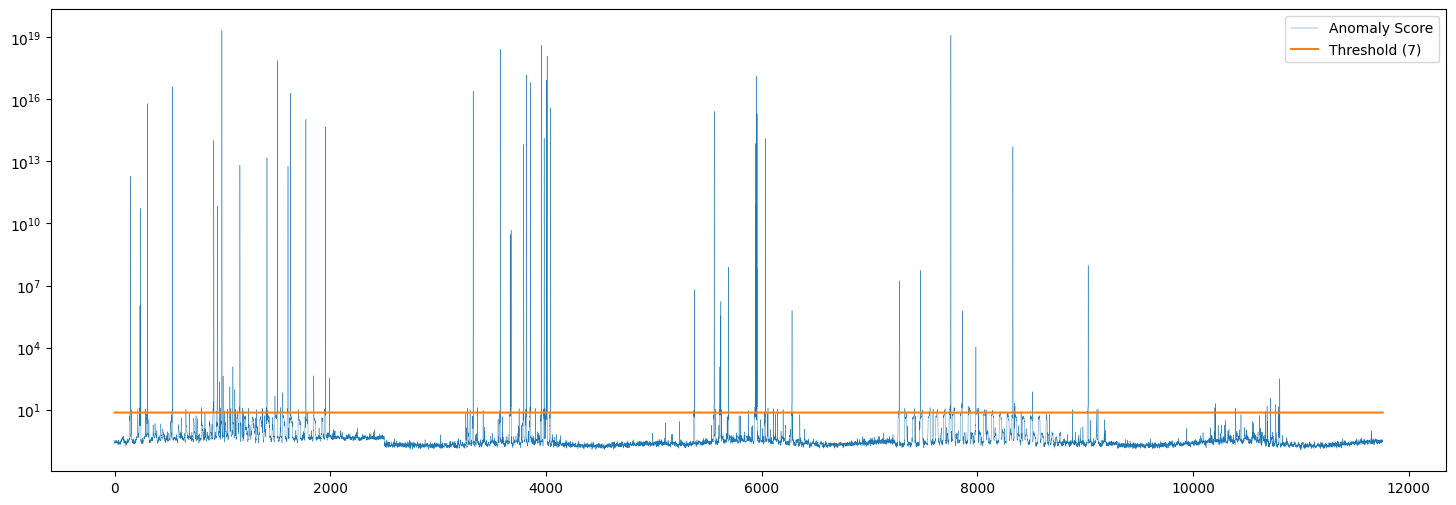
\includegraphics[width=1.3\textwidth]{figures/anomaly_scores_madgan_in.png}}
    \caption[Input Anomaly Scores]{Input Anomaly Scores. MAD-GAN Anomaly Reconstruction Scores for each profile in the input dataset. Profiles with scores above the orange line are considered anomalies.}
    % \label{fig:enter-label}
\end{figure}

\begin{figure}
    \makebox[\linewidth]{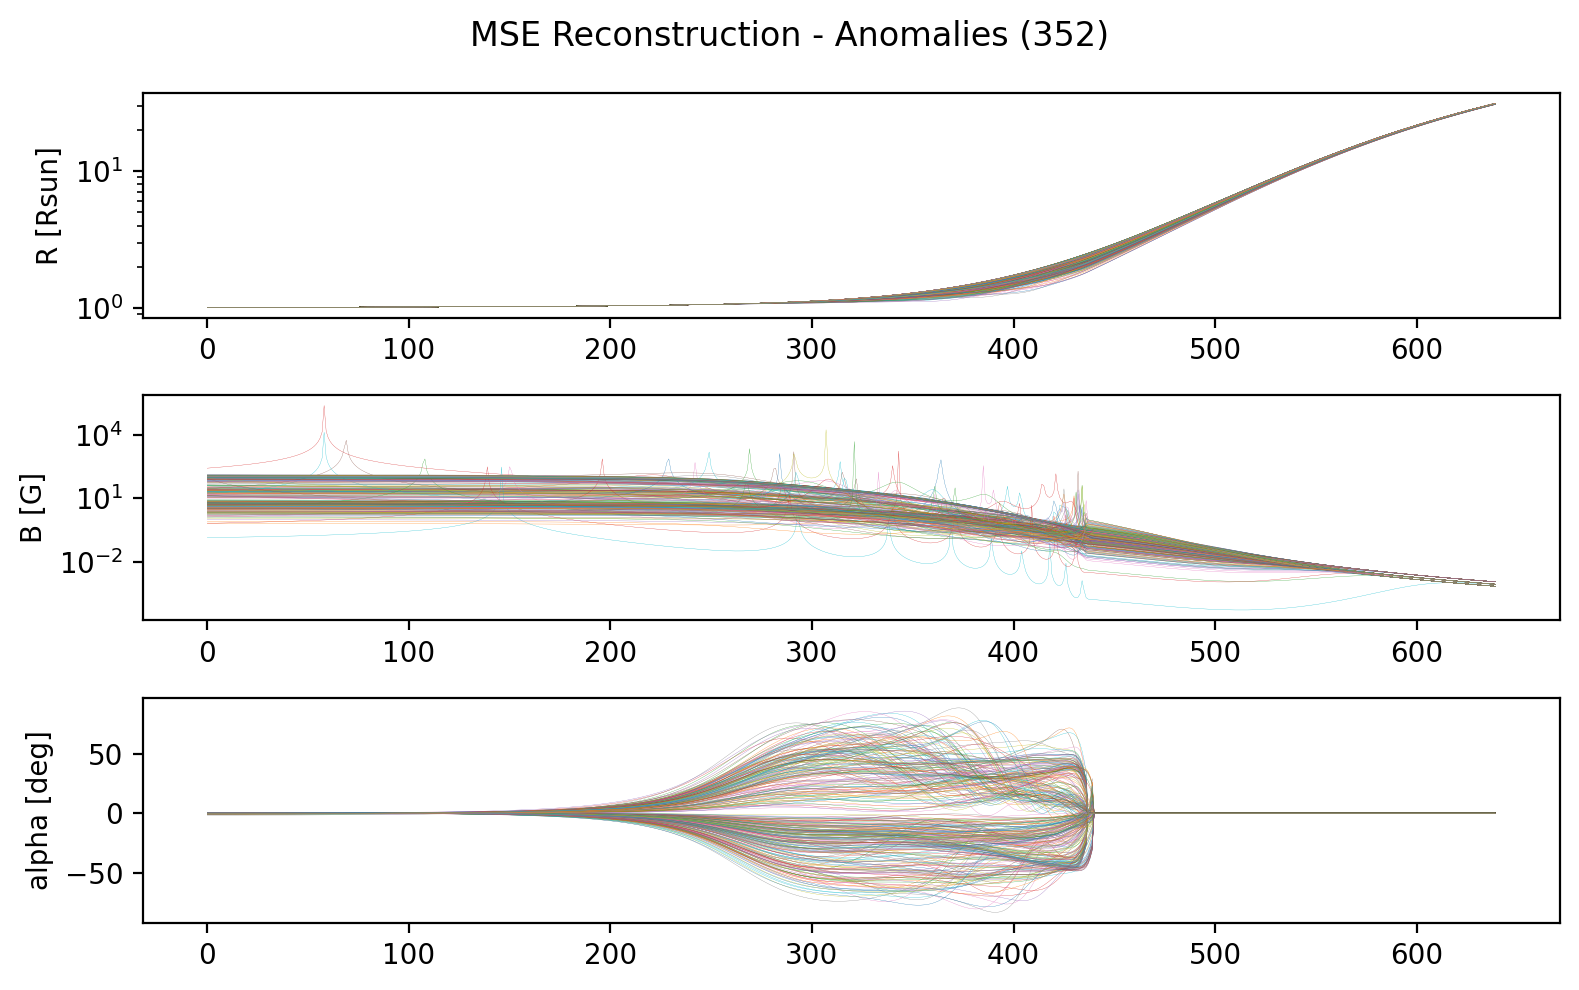
\includegraphics[width=1.2\linewidth]{figures/anomalies_madgan_in.png}}
    \caption{Anomalies detected with the MAD-GAN input model.}
    \label{fig_a:madgan_in_anomalies}
\end{figure}

\clearpage
\section{Output Model}

\begin{figure}[h]
    \centering
    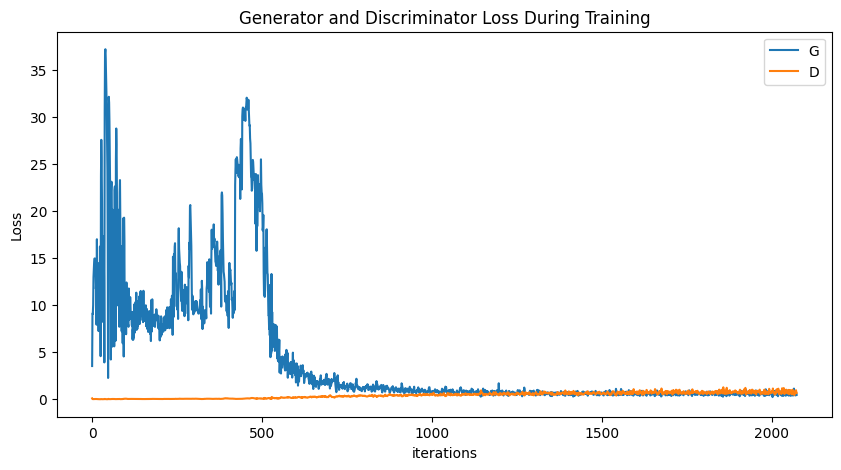
\includegraphics[width=0.8\textwidth]{figures/madgan_train_hist_out.png}
    \caption{MAD-GAN output model training history.}
    % \label{fig:enter-label}
\end{figure}

\begin{figure}
    \centering
    \rotatebox[origin=c]{-90}{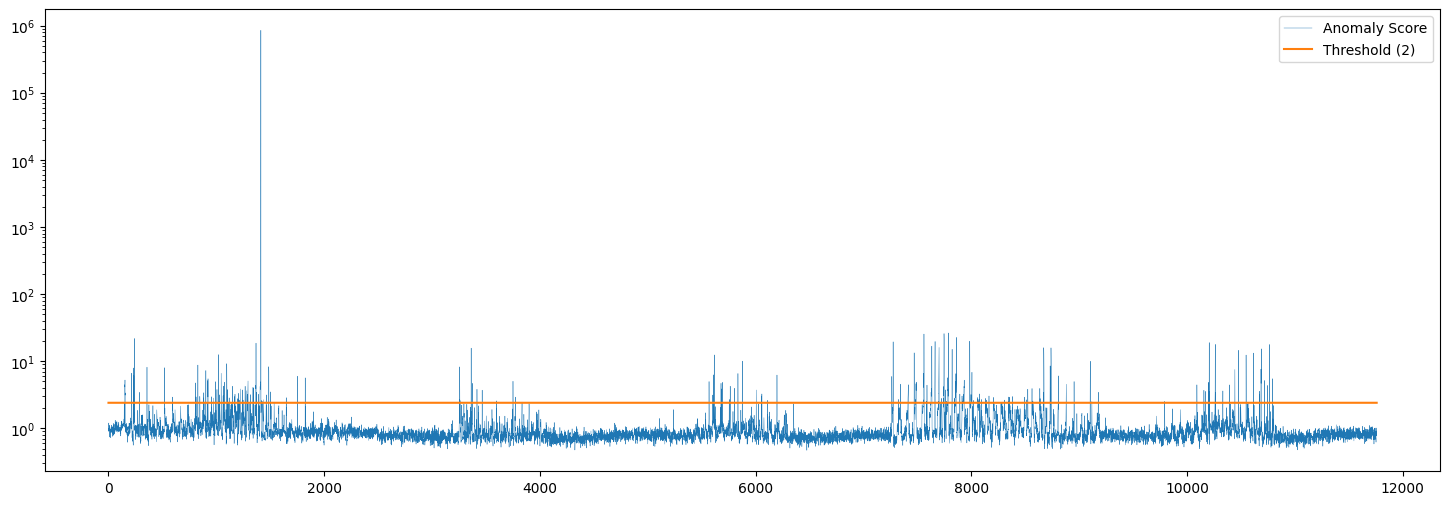
\includegraphics[width=1.3\textwidth]{figures/anomaly_scores_madgan_out.png}}
    \caption[Output Anomaly Scores]{Output Anomaly Scores. MAD-GAN Anomaly Reconstruction Scores for each profile in the output dataset. Profiles with scores above the orange line are considered anomalies.}
    % \label{fig:enter-label}
\end{figure}

\begin{figure}
    \centering
    \makebox[\linewidth]{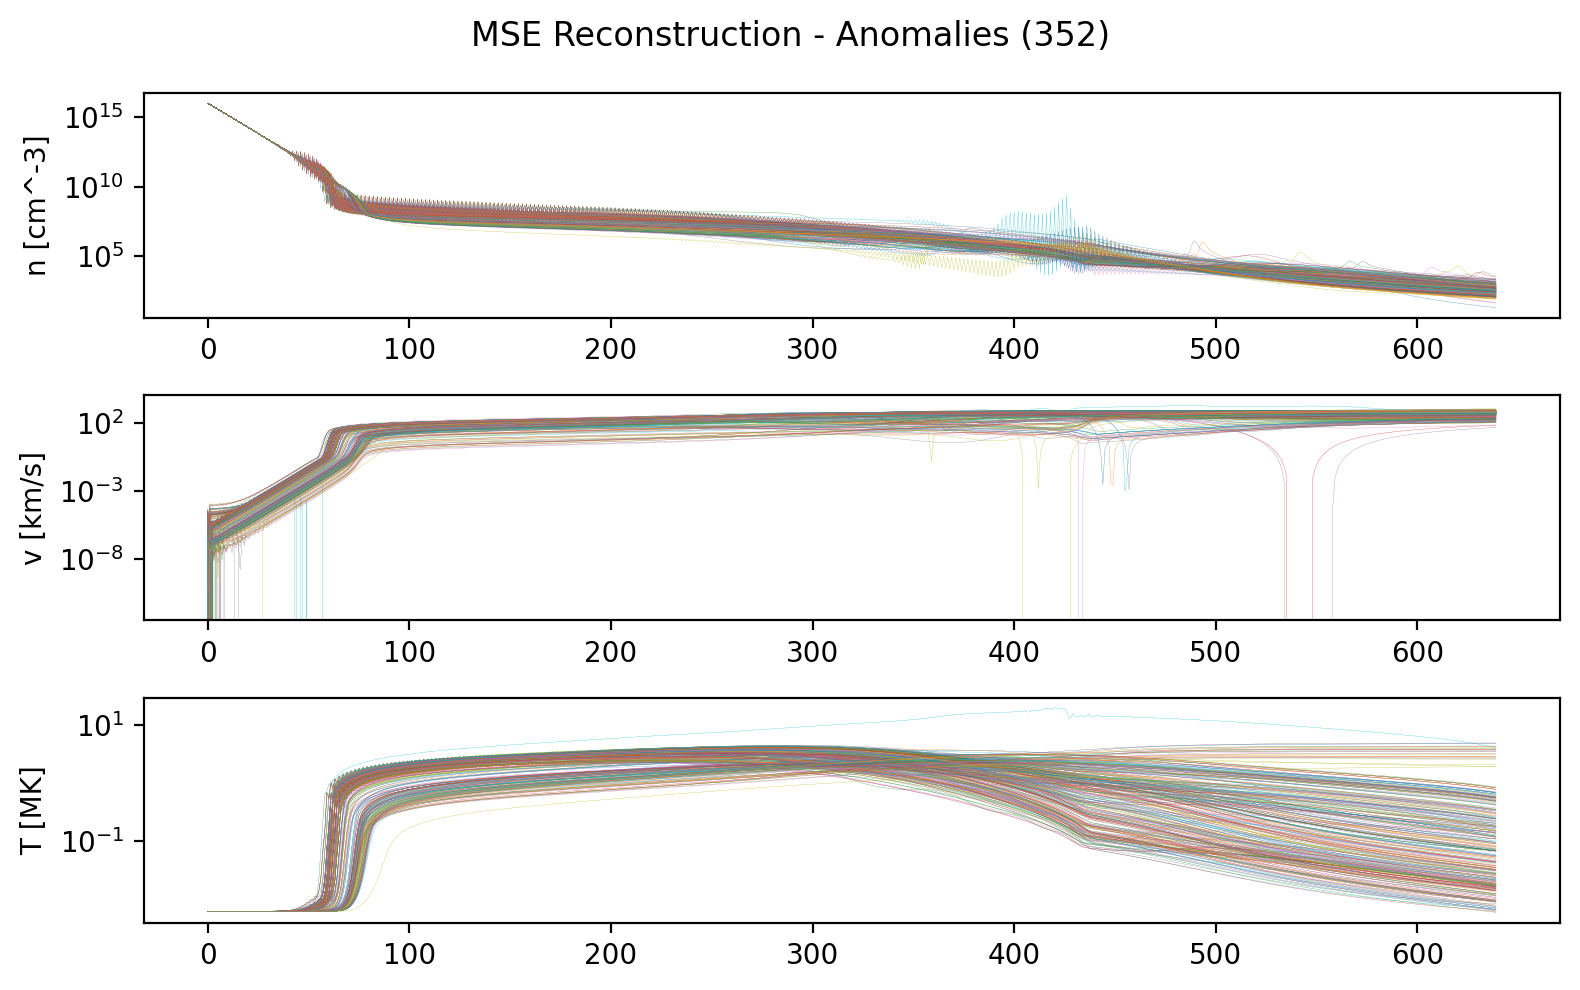
\includegraphics[width=1.2\linewidth]{figures/anomalies_madgan_out.png}
    \caption{Anomalies detected with the MAD-GAN output model.}}
    \label{fig:enter-label}
\end{figure}